% Presentation -- 12 slides. Compile with pdfLaTeX (Overleaf: upload this file, Recompile).
% Self-contained: diagrams and charts are drawn with TikZ/pgfplots, no image files.
% Every number comes from reports/*.md|json and PROJECT_SUMMARY.md in the repository.
\documentclass[aspectratio=169,11pt]{beamer}
\usetheme{Madrid}
\usepackage[T1]{fontenc}
\usepackage[utf8]{inputenc}
\usepackage{lmodern}
\usepackage{booktabs}
\usepackage{tikz}
\usetikzlibrary{arrows.meta,positioning}
\usepackage{pgfplots}
\pgfplotsset{compat=1.17}

\definecolor{accent}{HTML}{0E7490}
\definecolor{warn}{HTML}{B45309}
\definecolor{dronered}{HTML}{D6452A}
\definecolor{unkviolet}{HTML}{7A4FD6}
\definecolor{lowamber}{HTML}{D99A0B}
\definecolor{nogray}{HTML}{8A8984}
\setbeamercolor{structure}{fg=accent}
\setbeamercolor{palette primary}{bg=accent,fg=white}
\setbeamercolor{palette secondary}{bg=accent!80!black,fg=white}
\setbeamercolor{palette tertiary}{bg=accent!60!black,fg=white}
\setbeamercolor{title}{bg=accent,fg=white}
\setbeamercolor{frametitle}{bg=accent!10,fg=accent!70!black}
\setbeamercolor{block title alerted}{bg=warn,fg=white}
\setbeamercolor{block body alerted}{bg=warn!8}
\setbeamertemplate{navigation symbols}{}

\title[Counter-Drone Detection]{Counter-Drone Detection from Sound and Radio}
\subtitle{Acoustic + 2.4\,GHz RF detection with uncertainty and late fusion}
\author[Vidhi.R \& Kathan.D ]{Vidhi Rojasara (AU2644022) \and Kathan Desai (AU2644002)}
\institute[Ahmedabad University]{AI Lab --- Prof.\ Maitrik Shah\\Ahmedabad University, Ahmedabad}
\date{November 2026}

\begin{document}

% 1 ---------------------------------------------------------------------
\begin{frame}
  \titlepage
\end{frame}

% 2 ---------------------------------------------------------------------
\begin{frame}{Problem}
\begin{columns}[T]
\column{0.55\textwidth}
\begin{itemize}
  \item Small drones are cheap, quiet and hard to see: a risk for campuses, prisons, events.
  \item Detect them from \textbf{sound} (rotor noise) and their \textbf{2.4\,GHz radio link}.
  \item Hard part: wind, traffic, speech, music, helicopters; Wi-Fi and Bluetooth on the same band.
  \item Public benchmarks report scores near \textbf{1.0} --- often from \emph{one recording session},
        so a model can learn the room or receiver instead of the drone.
\end{itemize}
\column{0.42\textwidth}
\begin{alertblock}{Our question}
Build a detector, and measure honestly how well it works \textbf{outside} the conditions it was
trained on --- and say when it is unsure.
\end{alertblock}
\end{columns}
\end{frame}

% 3 ---------------------------------------------------------------------
\begin{frame}{Objectives}
\begin{enumerate}
  \item Leakage-safe data: slices of one recording never in two splits.
  \item Acoustic detector vs.\ baseline, CNN, CNN+GRU, CNN+LSTM, transformer.
  \item Tiered tests: same data $\rightarrow$ unseen drone $\rightarrow$ outdoor $\rightarrow$ outdoor + outdoor training.
  \item Noise robustness: voice, traffic, wind, real speech and music at 20/10/0\,dB.
  \item Four output states instead of yes/no: \textcolor{nogray}{\textbf{No Drone}},
        \textcolor{dronered}{\textbf{Known Drone}}, \textcolor{unkviolet}{\textbf{Unknown Drone}},
        \textcolor{lowamber}{\textbf{Low Confidence}}.
  \item RF detector, checked on a \textbf{second receiver}.
  \item Audio + RF fusion with a full ablation; Grad-CAM; dashboard.
\end{enumerate}
\end{frame}

% 4 ---------------------------------------------------------------------
\begin{frame}{Data}
\small
\begin{tabular}{@{}lll@{}}
\toprule
Dataset & Role & Size \\
\midrule
DroneAudioDataset + ESC-50 & Audio, indoor training & 1,332 drone / $\sim$10,370 background clips \\
ITU ARIS Lab & Audio, outdoor training & 4,491 drone / 1,000 background clips \\
Svanstr\"om & Audio, outdoor \textbf{test} & 30 drone / 30 helicopter / 30 background \\
DroneRF & RF & 227 segments, 3 drones + background, one lab \\
Tampere & RF, second receiver & 11 drones, anechoic chamber \\
AeroSonicDB & Outdoor aircraft check & 99 aircraft, 317 ambience recordings \\
\bottomrule
\end{tabular}
\vspace{6pt}
\begin{itemize}\small
  \item 18,093 audio clips in total; all cut to fixed 1\,s at 16\,kHz.
  \item Why: in the raw data, \textbf{clip duration alone} predicted the label (AUC 1.0).
\end{itemize}
\end{frame}

% 5 ---------------------------------------------------------------------
\begin{frame}{System architecture}
\centering
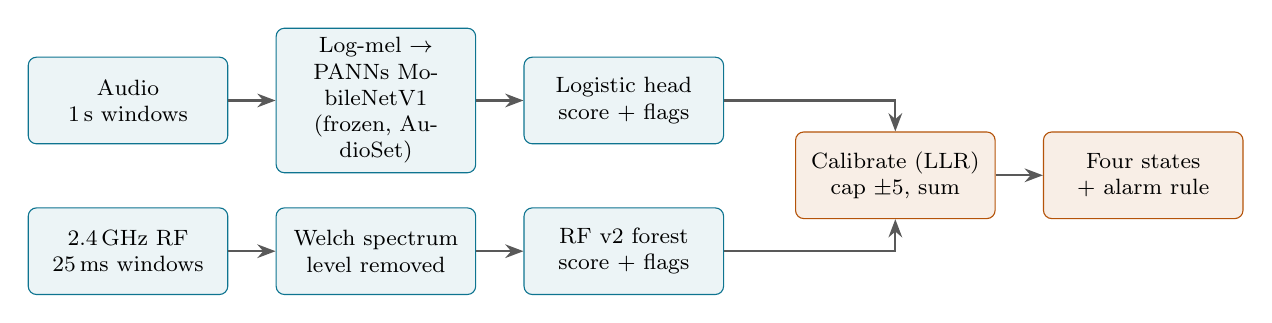
\begin{tikzpicture}[
  node distance=4mm and 6mm,
  box/.style={draw=accent, rounded corners=3pt, fill=accent!8, align=center,
              font=\footnotesize, minimum height=11mm, text width=23mm},
  dec/.style={draw=warn, rounded corners=3pt, fill=warn!10, align=center,
              font=\footnotesize, minimum height=11mm, text width=23mm},
  arr/.style={-Stealth, thick, draw=black!65}]
  \node[box] (mic) {Audio\\1\,s windows};
  \node[box, right=of mic] (enc) {Log-mel $\rightarrow$\\PANNs MobileNetV1\\(frozen, AudioSet)};
  \node[box, right=of enc] (head) {Logistic head\\score + flags};
  \node[box, below=8mm of mic] (rf) {2.4\,GHz RF\\25\,ms windows};
  \node[box, right=of rf] (psd) {Welch spectrum\\level removed};
  \node[box, right=of psd] (forest) {RF v2 forest\\score + flags};
  \node[dec, right=9mm of head, yshift=-9.5mm] (fuse) {Calibrate (LLR)\\cap $\pm$5, sum};
  \node[dec, right=of fuse] (state) {Four states\\+ alarm rule};
  \draw[arr] (mic) -- (enc); \draw[arr] (enc) -- (head);
  \draw[arr] (rf) -- (psd); \draw[arr] (psd) -- (forest);
  \draw[arr] (head) -| (fuse); \draw[arr] (forest) -| (fuse);
  \draw[arr] (fuse) -- (state);
\end{tikzpicture}
\vspace{8pt}
\begin{itemize}\small
  \item Each sensor keeps its own detector; late fusion of calibrated evidence (log-likelihood ratios).
  \item Explainability: Grad-CAM per window. Alarm after 2 consecutive drone windows.
  \item RF windows come from recorded datasets: \textbf{no live RF receiver}.
\end{itemize}
\end{frame}

% 6 ---------------------------------------------------------------------
\begin{frame}{Experiments: protocol and the four states}
\begin{columns}[T]
\column{0.5\textwidth}
\textbf{Evaluation protocol}
\begin{itemize}\small
  \item Split by \textbf{parent recording} (RF: time blocks); a validator stops on any leak.
  \item Tier 1 held-out recordings; Tier 2 unseen drone (Mambo); Tier 3 outdoor Svanstr\"om;
        Tier 4 + outdoor training.
  \item Threshold at \textbf{1\% false alarms on validation}, frozen for test.
  \item PR-AUC with recording-level 95\% CIs, recall, false-alarm rate.
\end{itemize}
\column{0.48\textwidth}
\textbf{Output states}
\begin{itemize}\small
  \item[\textcolor{nogray}{$\bullet$}] \textbf{No Drone}: evidence below threshold --- not proof of absence.
  \item[\textcolor{dronered}{$\bullet$}] \textbf{Known Drone}: resembles training drones (not a model ID).
  \item[\textcolor{unkviolet}{$\bullet$}] \textbf{Unknown Drone}: drone-like, unfamiliar signature.
  \item[\textcolor{lowamber}{$\bullet$}] \textbf{Low Confidence}: near threshold or unfamiliar input $\rightarrow$ human review.
\end{itemize}
\end{columns}
\end{frame}

% 7 ---------------------------------------------------------------------
\begin{frame}{Results: audio across tiers}
\begin{columns}[c]
\column{0.55\textwidth}
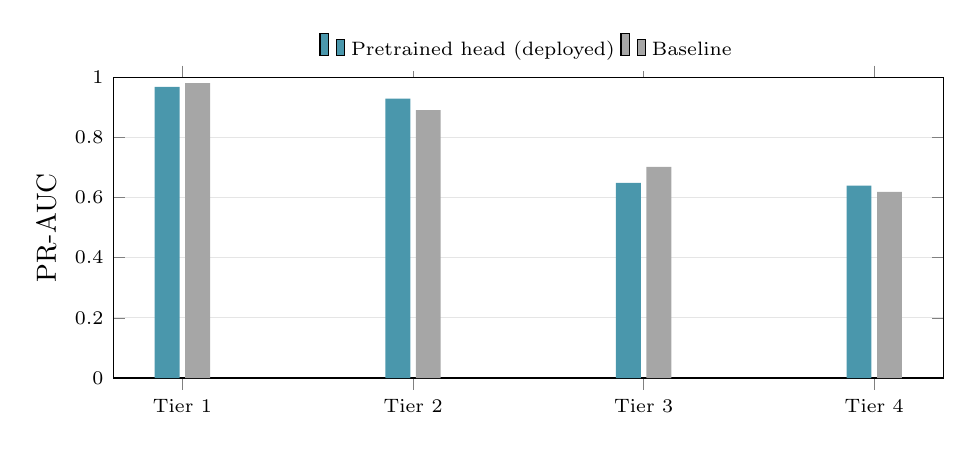
\begin{tikzpicture}
\begin{axis}[ybar, bar width=9pt, width=\linewidth, height=5.4cm, ymin=0, ymax=1,
  ylabel={PR-AUC}, symbolic x coords={Tier 1,Tier 2,Tier 3,Tier 4}, xtick=data,
  legend style={at={(0.5,1.02)}, anchor=south, legend columns=2, font=\scriptsize, draw=none},
  ymajorgrids, grid style={black!10}, tick label style={font=\scriptsize}]
\addplot[fill=accent!75, draw=none] coordinates {(Tier 1,0.968) (Tier 2,0.929) (Tier 3,0.649) (Tier 4,0.640)};
\addplot[fill=black!35, draw=none] coordinates {(Tier 1,0.981) (Tier 2,0.891) (Tier 3,0.702) (Tier 4,0.619)};
\legend{Pretrained head (deployed), Baseline}
\end{axis}
\end{tikzpicture}
\column{0.43\textwidth}
\begin{itemize}\small
  \item Indoors: PR-AUC \textbf{0.968}.
  \item Outdoors (tier 4): catches \textbf{22\%} of drone windows (66/300) at 1\% false alarms (6/600).
  \item Per recording: \textbf{14/30} drones alarmed, 1/30 helicopters, 0/30 background.
  \item Main confusion: helicopters (drone vs helicopter AUC $\approx$0.58).
\end{itemize}
\end{columns}
\end{frame}

% 8 ---------------------------------------------------------------------
\begin{frame}{Results: model comparison and noise}
\begin{columns}[T]
\column{0.5\textwidth}
\textbf{Outdoor PR-AUC (tier 3)}\\[2pt]
\small
\begin{tabular}{@{}lc@{}}
\toprule
Model & PR-AUC \\
\midrule
\textbf{CNN (from scratch, 211k)} & \textbf{0.831} \\
CNN+GRU & 0.810 \\
Transformer & 0.702 \\
Baseline & 0.702 \\
Pretrained head (deployed) & 0.649 \\
\bottomrule
\end{tabular}\\[4pt]
\footnotesize CNN separates drone vs helicopter at 0.911. Transformer best on unseen drone (recall 0.716).
\column{0.48\textwidth}
\textbf{Noise at 0\,dB SNR (recall)}\\[2pt]
\footnotesize
\begin{tabular}{@{}lcc@{}}
\toprule
Noise & Pretrained & + augmentation \\
\midrule
Clean & 0.878 & 0.882 \\
Real speech & 0.269 & \textbf{0.584} \\
Real music & 0.449 & \textbf{0.559} \\
Traffic & 0.502 & 0.547 \\
Wind & 0.743 & 0.796 \\
\bottomrule
\end{tabular}\\[4pt]
Augmentation helps in every condition. Loud music causes 7--9\% false alarms.
\end{columns}
\end{frame}

% 9 ---------------------------------------------------------------------
\begin{frame}{Results: the RF shortcut, and the fix}
\begin{columns}[T]
\column{0.47\textwidth}
\textbf{RF v1} (DroneRF only): PR-AUC \textbf{1.000} --- but
\begin{itemize}\small
  \item windows with \emph{no transmission} still separated at AUC 1.000;
  \item on a second receiver it called \textbf{100\% of pure noise ``drone''}.
\end{itemize}
It learned the \emph{recording session}, not the drone.\\[4pt]
\textbf{RF v2}: same features, fixed training data (relabelled silence, receiver-noise negatives,
second-receiver drones).
\column{0.5\textwidth}
\small
\begin{tabular}{@{}lcc@{}}
\toprule
Check & v1 & v2 \\
\midrule
Noise called drone (worst) & 1.000 & \textbf{0.080} \\
White-noise control & 1.000 & \textbf{0.000} \\
Unseen Tampere drones & n/a & \textbf{0.954} \\
Test: caught / false alarms & --- & 289/291, 4/390 \\
Left-out Phantom & 0.976 & 0.024 \\
\bottomrule
\end{tabular}\\[4pt]
\footnotesize Real Wi-Fi/Bluetooth false alarms are still unmeasured.
\end{columns}
\end{frame}

% 10 --------------------------------------------------------------------
\begin{frame}{Results: fusion ablation (unpaired pairs)}
\begin{columns}[c]
\column{0.55\textwidth}
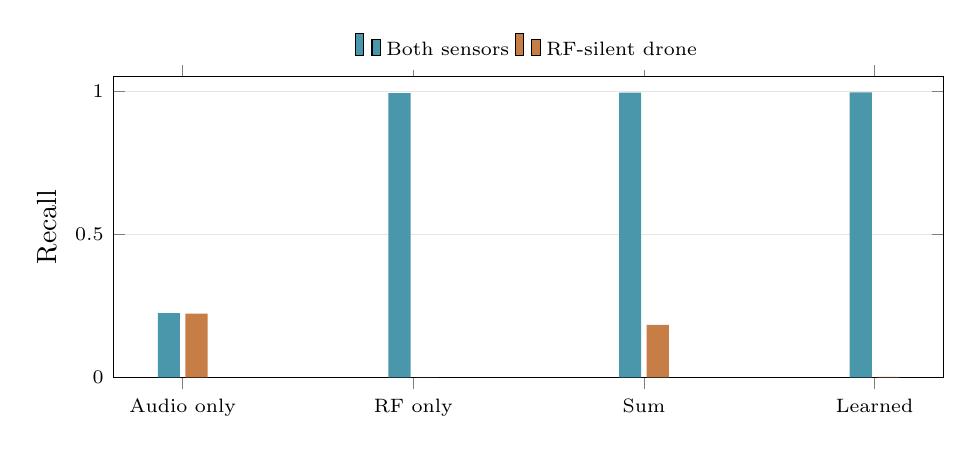
\begin{tikzpicture}
\begin{axis}[ybar, bar width=8pt, width=\linewidth, height=5.4cm, ymin=0, ymax=1.05,
  ylabel={Recall}, symbolic x coords={Audio only,RF only,Sum,Learned}, xtick=data,
  legend style={at={(0.5,1.02)}, anchor=south, legend columns=2, font=\scriptsize, draw=none},
  ymajorgrids, grid style={black!10}, tick label style={font=\scriptsize}]
\addplot[fill=accent!75, draw=none] coordinates {(Audio only,0.225) (RF only,0.993) (Sum,0.995) (Learned,0.996)};
\addplot[fill=warn!75, draw=none] coordinates {(Audio only,0.223) (RF only,0.0) (Sum,0.184) (Learned,0.002)};
\legend{Both sensors, RF-silent drone}
\end{axis}
\end{tikzpicture}
\column{0.43\textwidth}
\begin{itemize}\small
  \item Both sensors: fusion $\approx$ RF alone (RF's best case, one lab).
  \item \textbf{RF-silent drone:} sum keeps 0.184; the learned layer drops to \textbf{0.002}
        $\Rightarrow$ \textbf{evidence sum deployed}.
  \item Helicopter false alarms: 0.014 $\rightarrow$ 0.011 (sum).
\end{itemize}
\begin{alertblock}{Upper bound}
\footnotesize No dataset records audio and RF of the same flight: pairs are drawn independently.
\end{alertblock}
\end{columns}
\end{frame}

% 11 --------------------------------------------------------------------
\begin{frame}{Analysis: what the results show --- and do not}
\begin{columns}[T]
\column{0.48\textwidth}
\textbf{Show}
\begin{itemize}\small
  \item Audio works indoors and on an unseen drone.
  \item Outdoors it catches about a fifth of drone windows at 1\% false alarms.
  \item A near-perfect RF benchmark score was a session shortcut; v2 removes it.
  \item Uncertainty flags catch 80\% of indoor errors.
  \item No alarms on 99 real aircraft (AeroSonicDB).
\end{itemize}
\column{0.48\textwidth}
\textbf{Do not show}
\begin{itemize}\small
  \item Field performance at a real site.
  \item Synchronized audio+RF performance.
  \item RF false alarms on real Wi-Fi/Bluetooth.
  \item Calibrated audio probabilities.
\end{itemize}
\vspace{4pt}
\textbf{Demo}: \texttt{streamlit run app/dashboard.py} --- briefing, replay with the result first,
Grad-CAM, fusion ablation; \texttt{python -m console} for live microphone input.
\end{columns}
\end{frame}

% 12 --------------------------------------------------------------------
\begin{frame}{Conclusion and future work}
\begin{itemize}
  \item End-to-end acoustic drone detector with leakage-controlled, tiered evaluation and
        four-state uncertainty output; 182 automated tests.
  \item Key finding: benchmark scores near 1.0 did \textbf{not} survive a second receiver or the
        move outdoors --- we found the shortcut, fixed RF, and report the outdoor gap honestly.
\end{itemize}
\vspace{4pt}
\textbf{Next steps}
\begin{enumerate}\small
  \item Deploy the from-scratch CNN (best outdoor model); re-fit the uncertainty flags.
  \item Real Wi-Fi/Bluetooth RF negatives outside the DroneRF lab.
  \item Synchronized audio + RF recordings of the same flights.
  \item RF receiver (SDR) integration and field recordings.
\end{enumerate}
\vspace{4pt}
\centering\large\textbf{Thank you --- questions?}
\end{frame}

\end{document}
